\documentclass[
logosetup=topbar 
portrait,
%landscape,
a0paper%,
%draft
]
{baposter}
\usepackage{varwidth}
\usepackage{graphicx}
\usepackage{tikz,pgfplots}

\usepackage{relsize}
\usepackage[detect-weight]{siunitx}
 
\usepackage{booktabs}
\usepackage{amsmath}
\usepackage{float}
\usepackage{layouts}
\usepackage{multirow}
\usepackage{subfig}
\newcommand\e{\cdot 10^}
\setlength{\unitlength}{1.0cm}

\usepackage{xcolor,colortbl}

%\definecolor{hzbblue}{HTML}{0BA1E2}%{2E9EDC}%{1F95D6}
\definecolor{hzbblue}{RGB}{31,149,213}
\usepackage[scaled]{helvet}
\renewcommand*\familydefault{\sfdefault}
\usepackage[T1]{fontenc}

\renewcommand{\refname}{}

\usepackage{transparent}

\begin{document}
%
\begin{poster}{
grid=false,%true,
background=plain,
bgColorOne=white,
columns=3,
eyecatcher=true,
borderColor=hzbblue,
headerColorOne=white,
headershade=plain,
%headerColorTwo=hzbblue,
textborder=rounded,%none,%rectangle,
headerborder=open,
headershape=smallrounded,
headerfont=\bf\Large,
boxshade=none,
headerFontColor=hzbblue
}
{

\includegraphics[width=150pt]{berkeley/ucberkeleybluehex.pdf} 
}
{
\color{hzbblue}Streak camera setup and testing + tune resonance program developement at the MLS
}
{
\color{hzbblue} Levon Dovlatyan, Markus Ries, Paul Goslawski, and friends at HZB \\
\color{hzbblue} levondov@berkeley.edu
}
{

\includegraphics[width=100pt]{Pics/hzb_logo_clean.pdf} 
}
\headerbox{Introduction}{name=introbox,column=0,row=0,span=3}
{
\begin{tikzpicture}
\node at (0,4.5)[]{
\begin{varwidth}{10cm}
The Metrology Light Source (MLS) is an electron storage ring designed as a dedicated UV and VUV source; it has an asymmetric double-bend achromate design as well as a U180 undulator in one of its long straight sections. Radiation from this undulator as well as the magnets was used in initial test measurements of the bunch lengths with a new streak camera.
\end{varwidth}
};
\node at (0,1){
\begin{varwidth}{10cm}
However, the new streak camera's arrival was delayed for a few weeks because of manufacturing problems; this allowed time to develope a tune resonance program to be used mainly at the MLS. The program is written in python making it much easier to integrate with the systems at Bessy II (HZB) and the MLS (PTB).
\end{varwidth}
};
\node at (14.0,3) {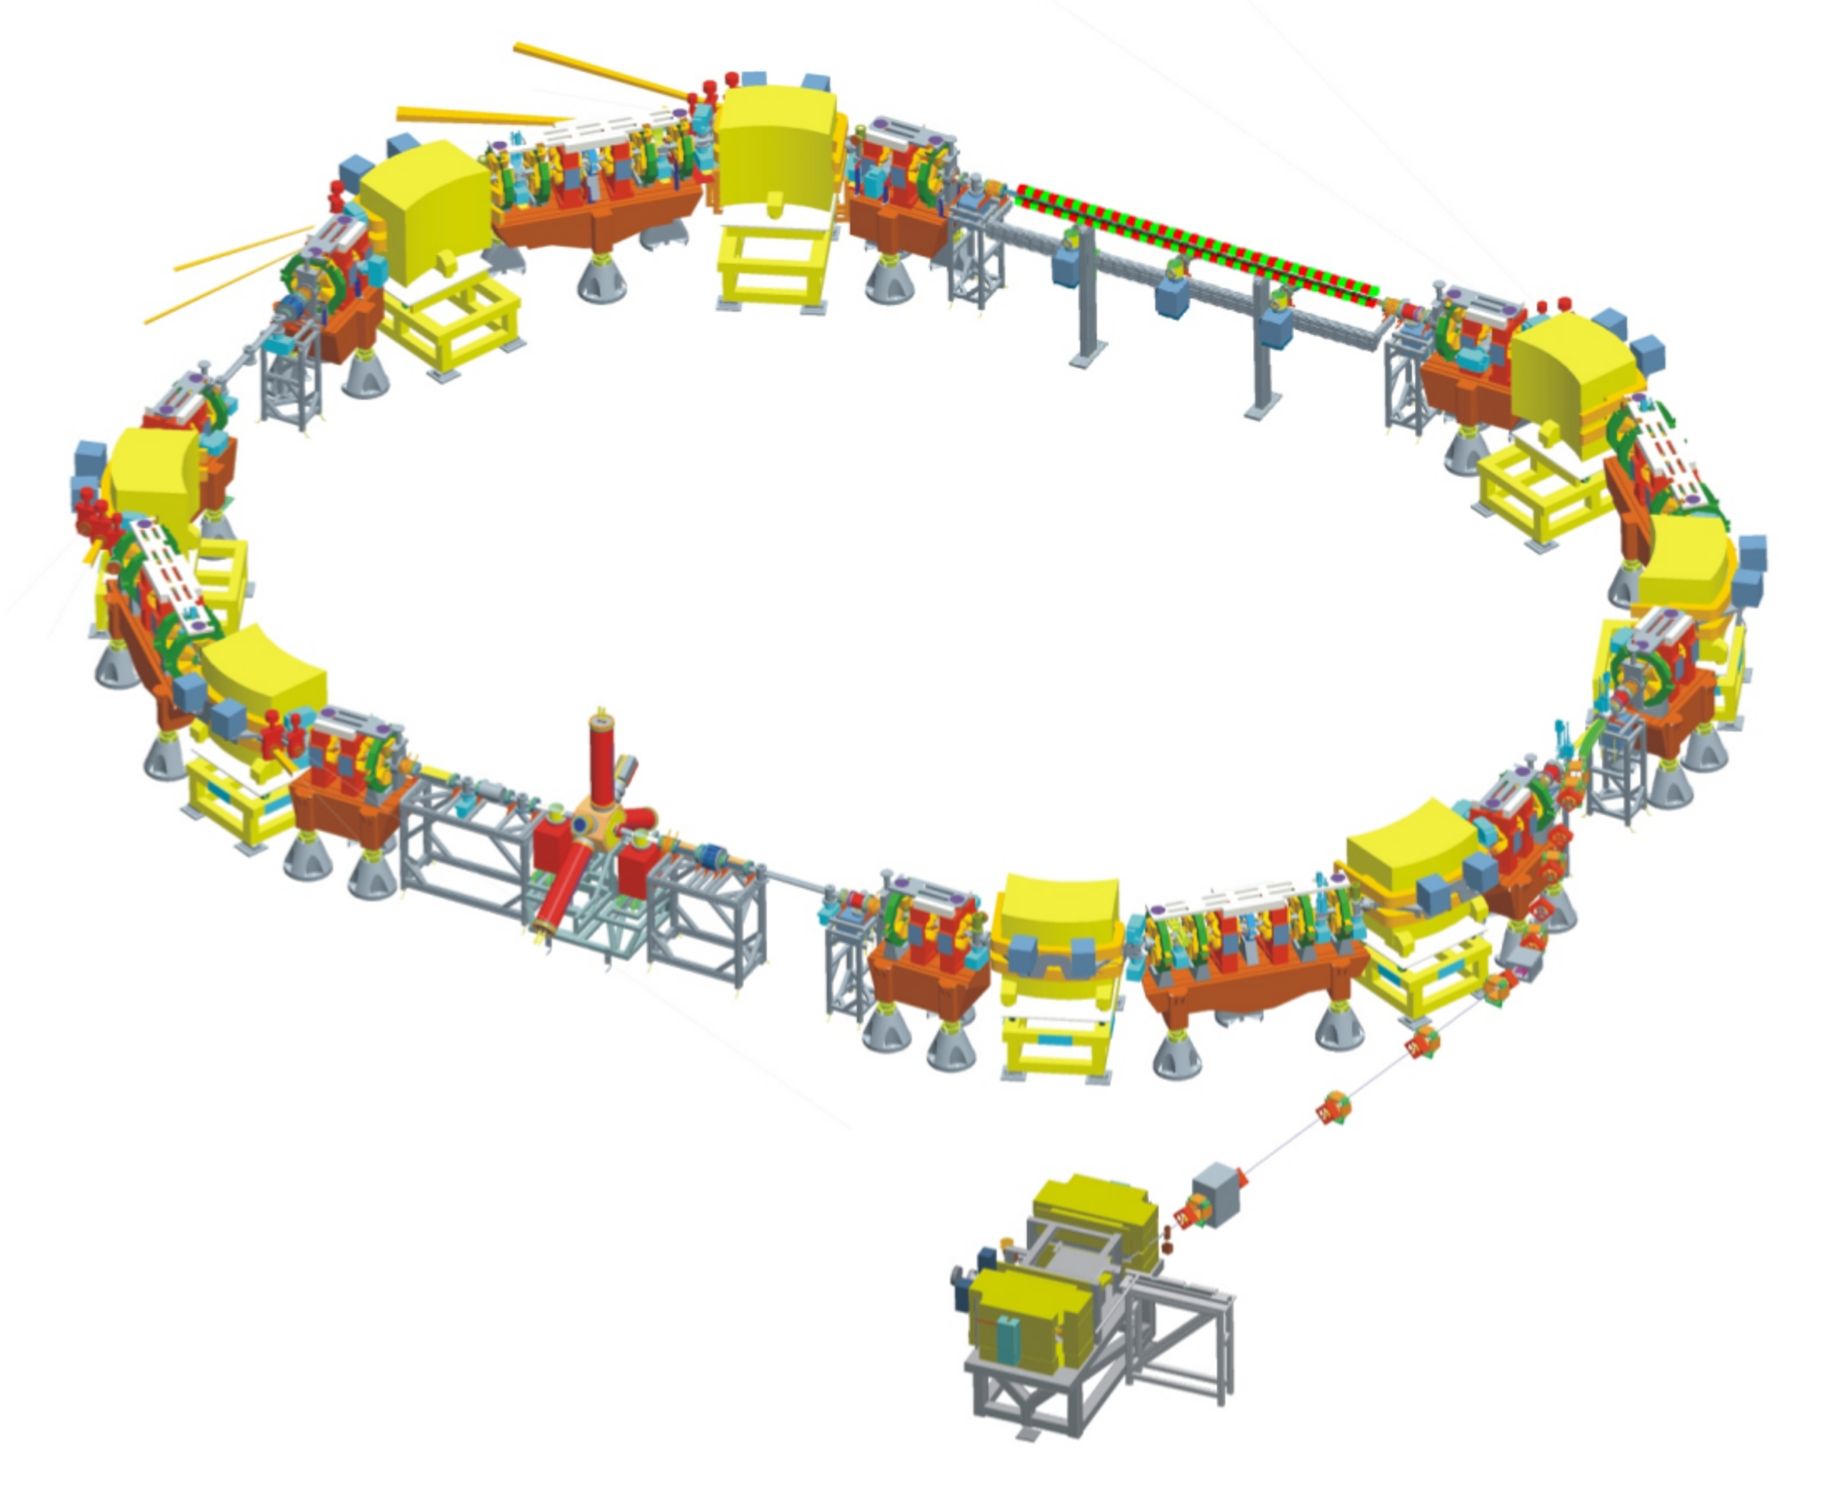
\includegraphics[width=250pt]{Pics/mls.pdf}};
\node at (10.5,0) {\footnotesize
\begin{tabular}{lc}%\hline
Lattice & {DBA}\\
Energy range / \si{\mega\electronvolt} &  105 to 630\\
Circumference / \si{\metre} &  48\\
Characteristic wavelength / \si{\nano\metre} &  3.4 to 735 \\
Tunes hor./ver. & {3.18 / 2.23}\\
Current$\times$Lifetime / \si{\ampere\hour}&  0.9  \\%\\\hline
electron beam current & 1 pA to 200 mA
\end{tabular}%
};
\node at (14,3.8){
\Huge\color{hzbblue} MLS
};
\node at (7.5,4){\fbox{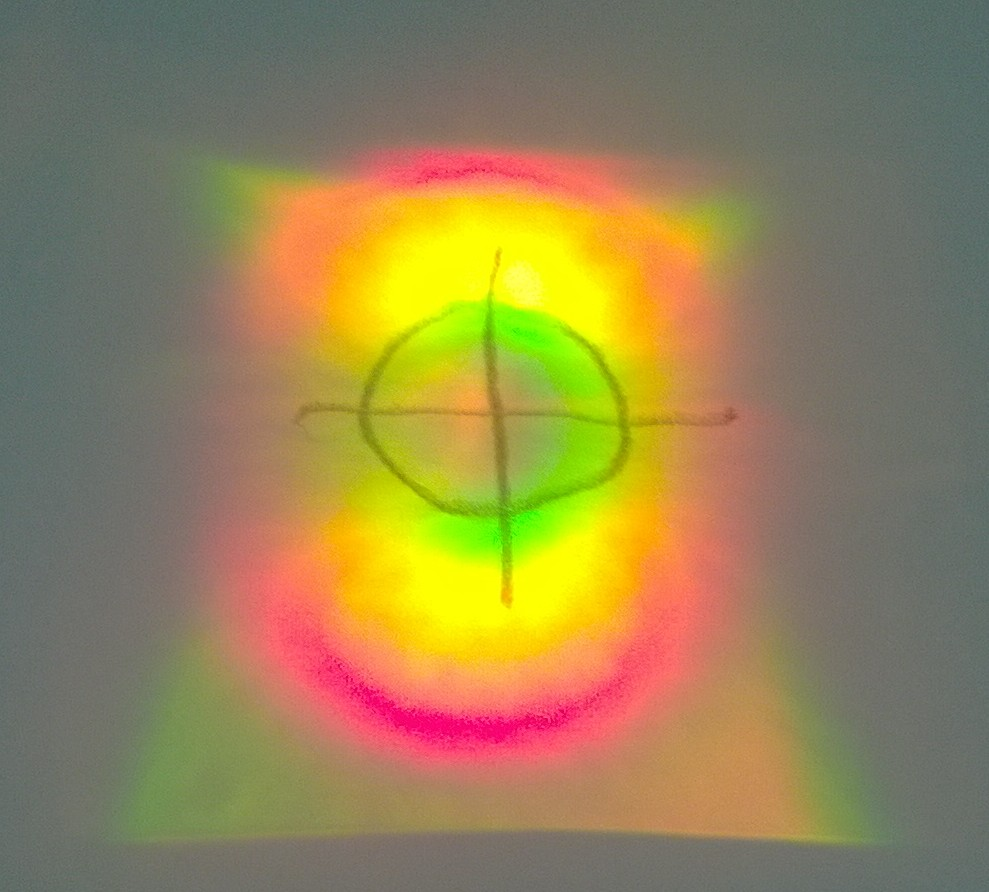
\includegraphics[width=100pt]{Pics/beam}}
};
\node at (7.5,2){
Beam used for alignment
};
\node at (17, -0.4){
\includegraphics[width=50pt]{Pics/PTB-Logo.pdf}};
%\draw[<->,thick] (1.3,3.75) -- node[midway,below] {$\Delta
%x\propto\eta_x$} (3.7,3.75);
\end{tikzpicture}
}

\headerbox{Streak Camera}{name=firstbox,below=introbox,column=0,row=1,span=2,above=bottom}
{
{\color{hzbblue}\bf\large Setup} \\[0.5cm]
\begin{tikzpicture}

\node at (1,0) {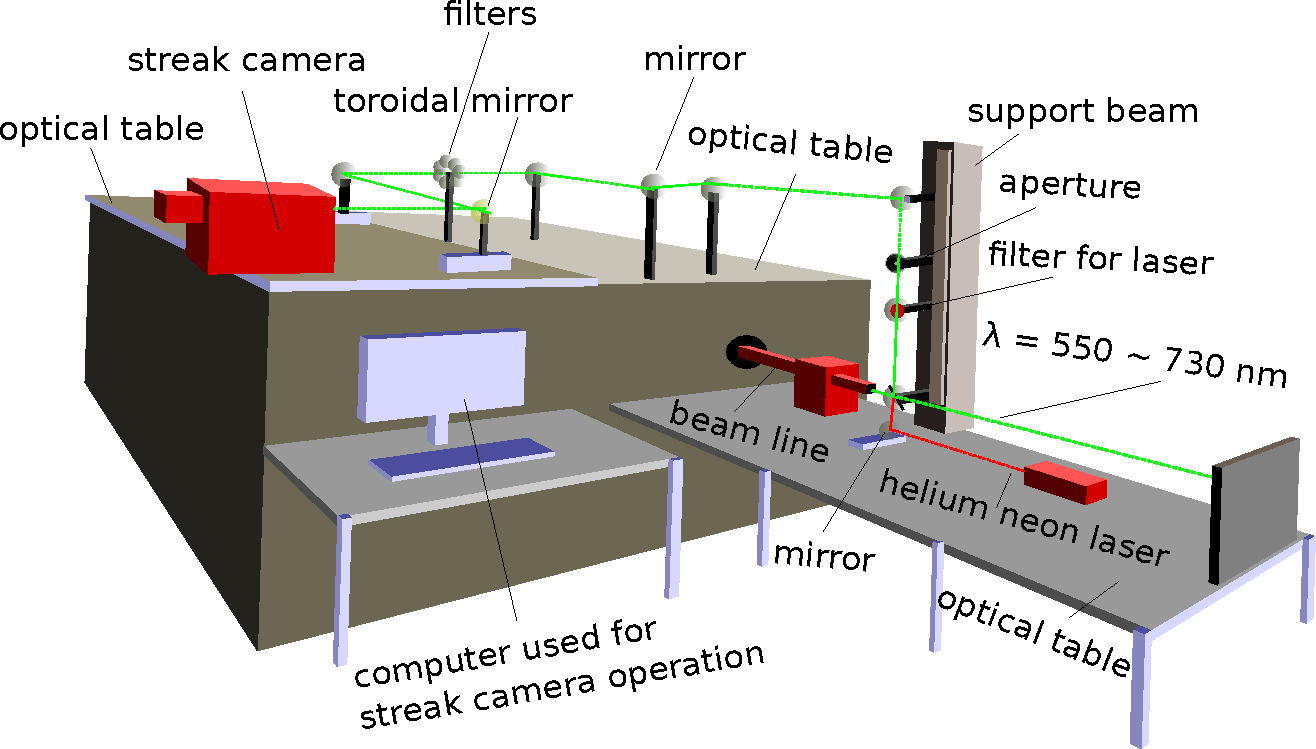
\includegraphics[width=350pt]{Pics/diagramtext.pdf}
};
\node at (8.7,0) {\fbox{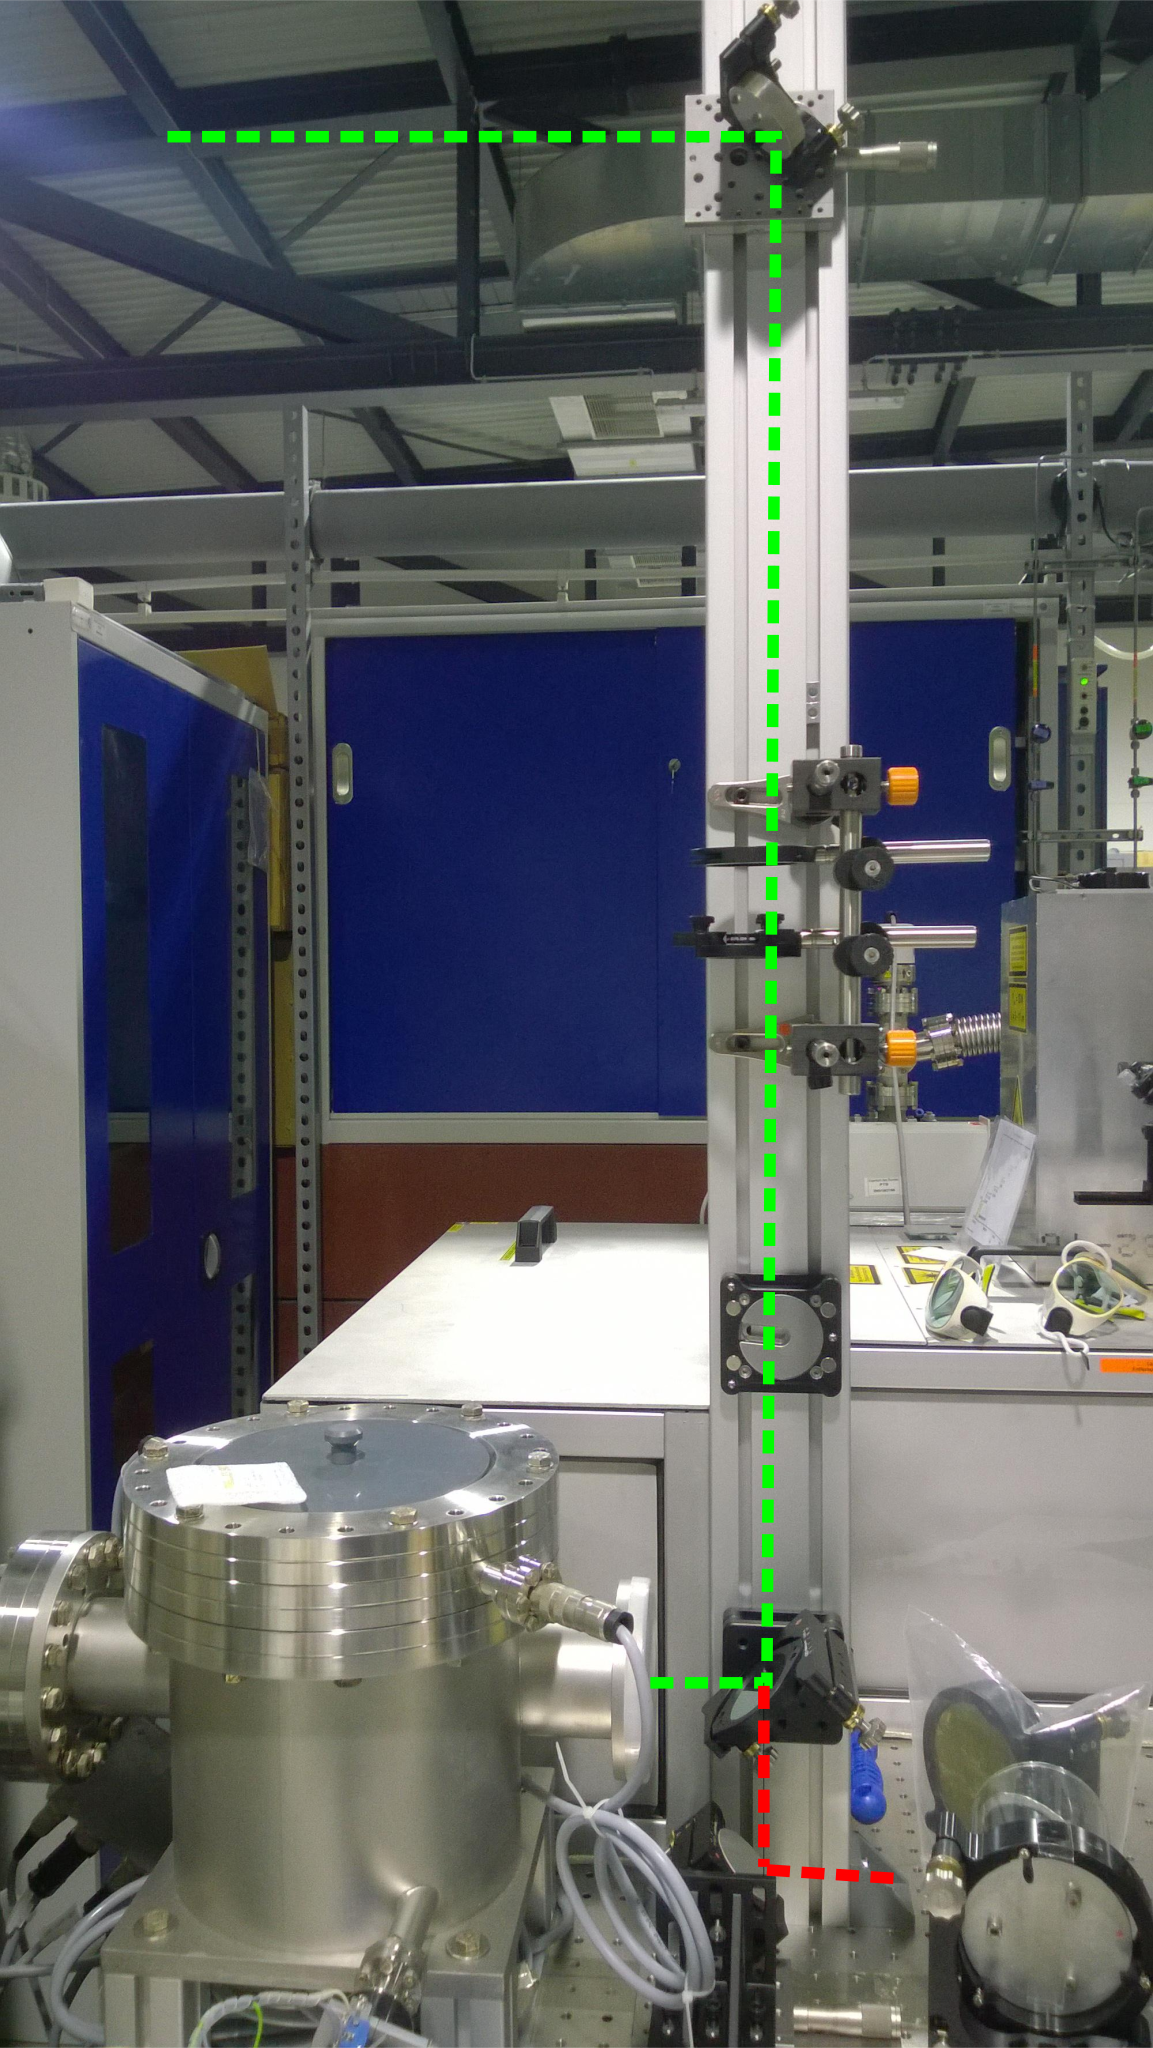
\includegraphics[width=75pt]{Pics/verticalbeam.pdf}}
};
\node at (6,-5.2) {\fbox{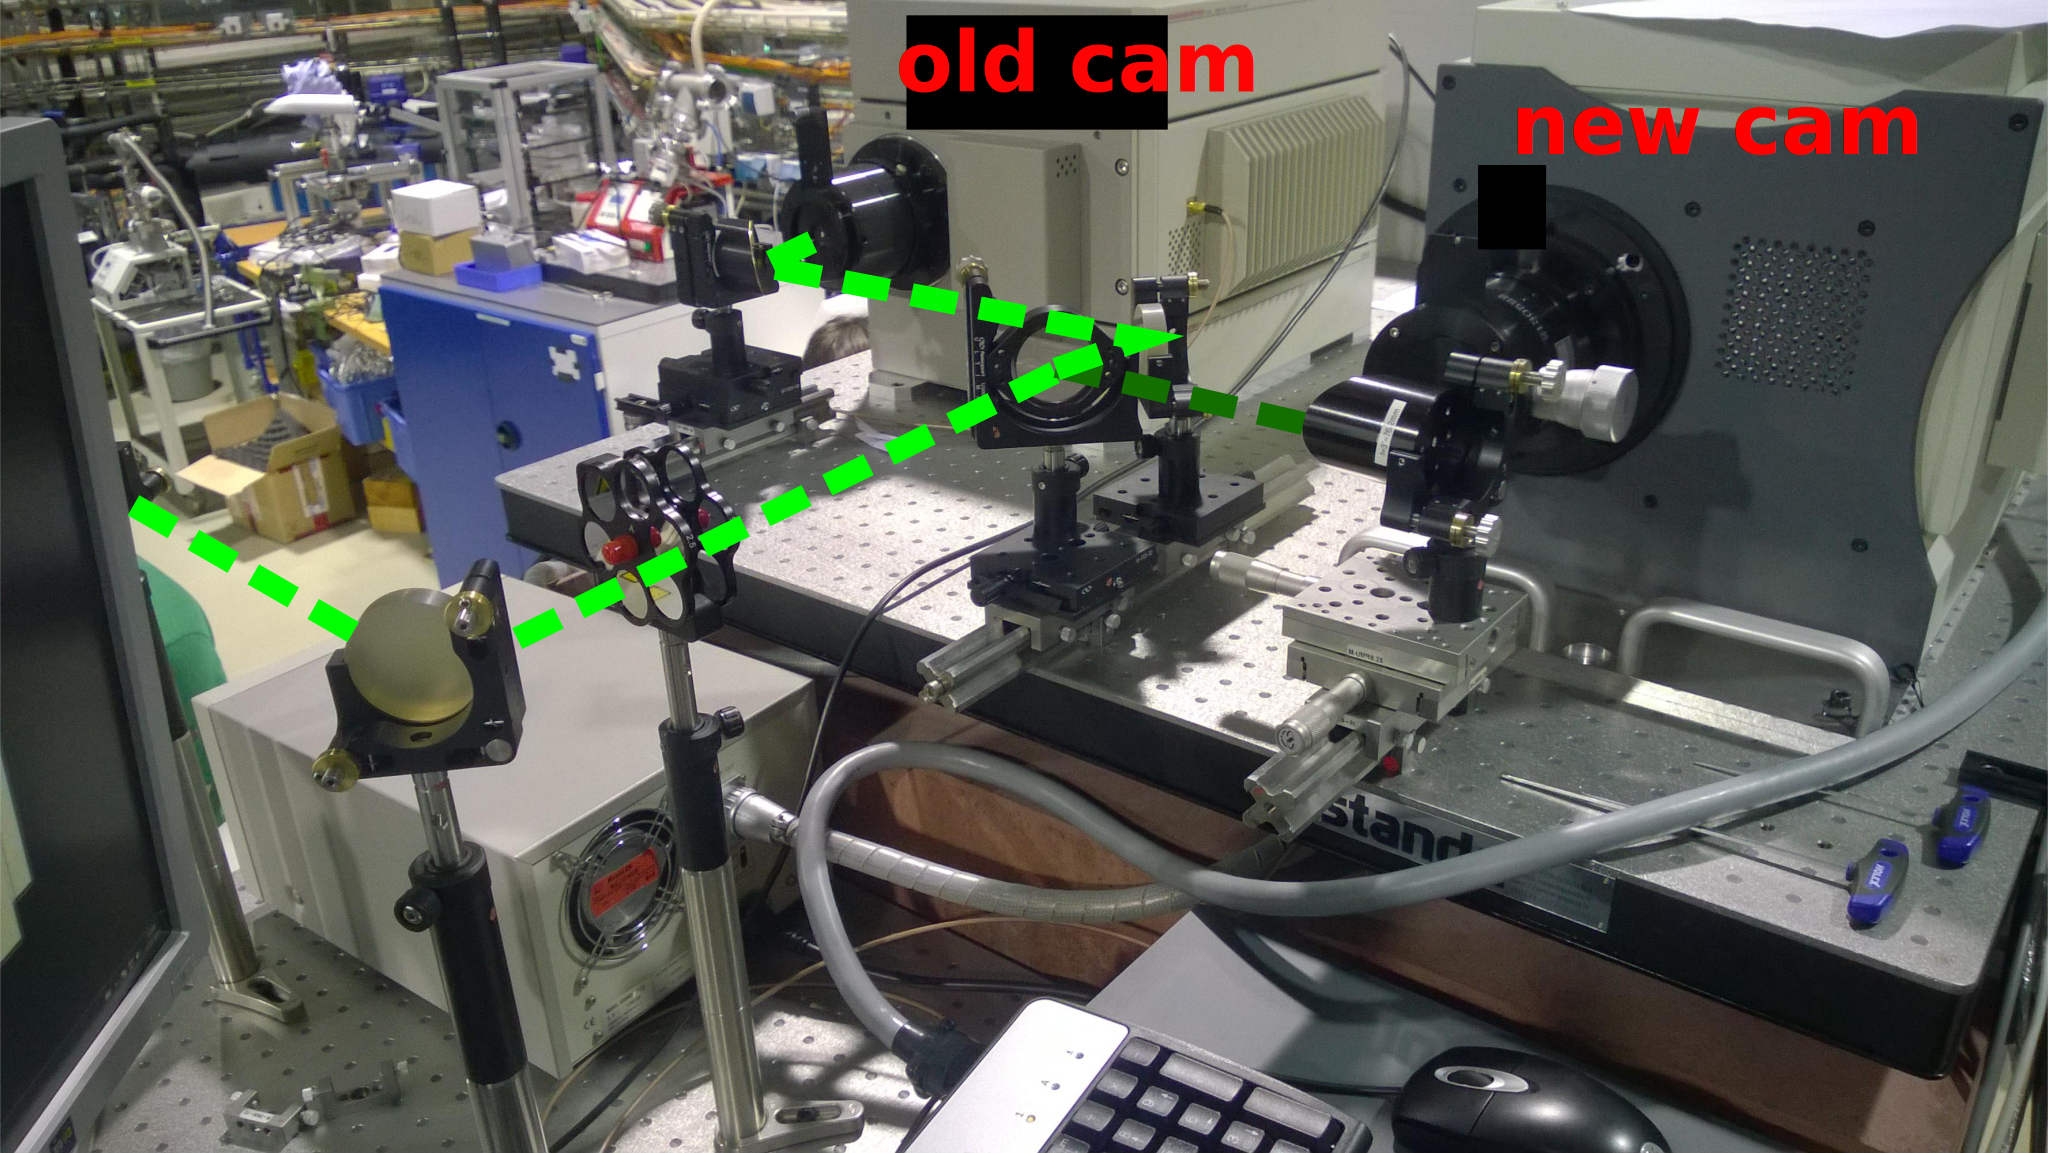
\includegraphics[width=150pt]{Pics/horizontaltable.pdf}}
};
\node at (6,-3.3) {
optical table setup for dual streak camera operation
};
\node at (8.7,2.7) {
support beam
};
\node at (-1,-5) {
\begin{varwidth}{7cm}
The toroidal mirrors, along with a splitter and a normal mirror, on the optical table are placed on rail systems in order to provide multiple degrees of freedom to adjust for the horizontal and vertical focuses of the beam
\end{varwidth}
};
\end{tikzpicture}


{\color{hzbblue}\bf\large Measurements} \\[0.5cm]
\begin{tikzpicture}[]

\node at (0,3.3) {\fbox{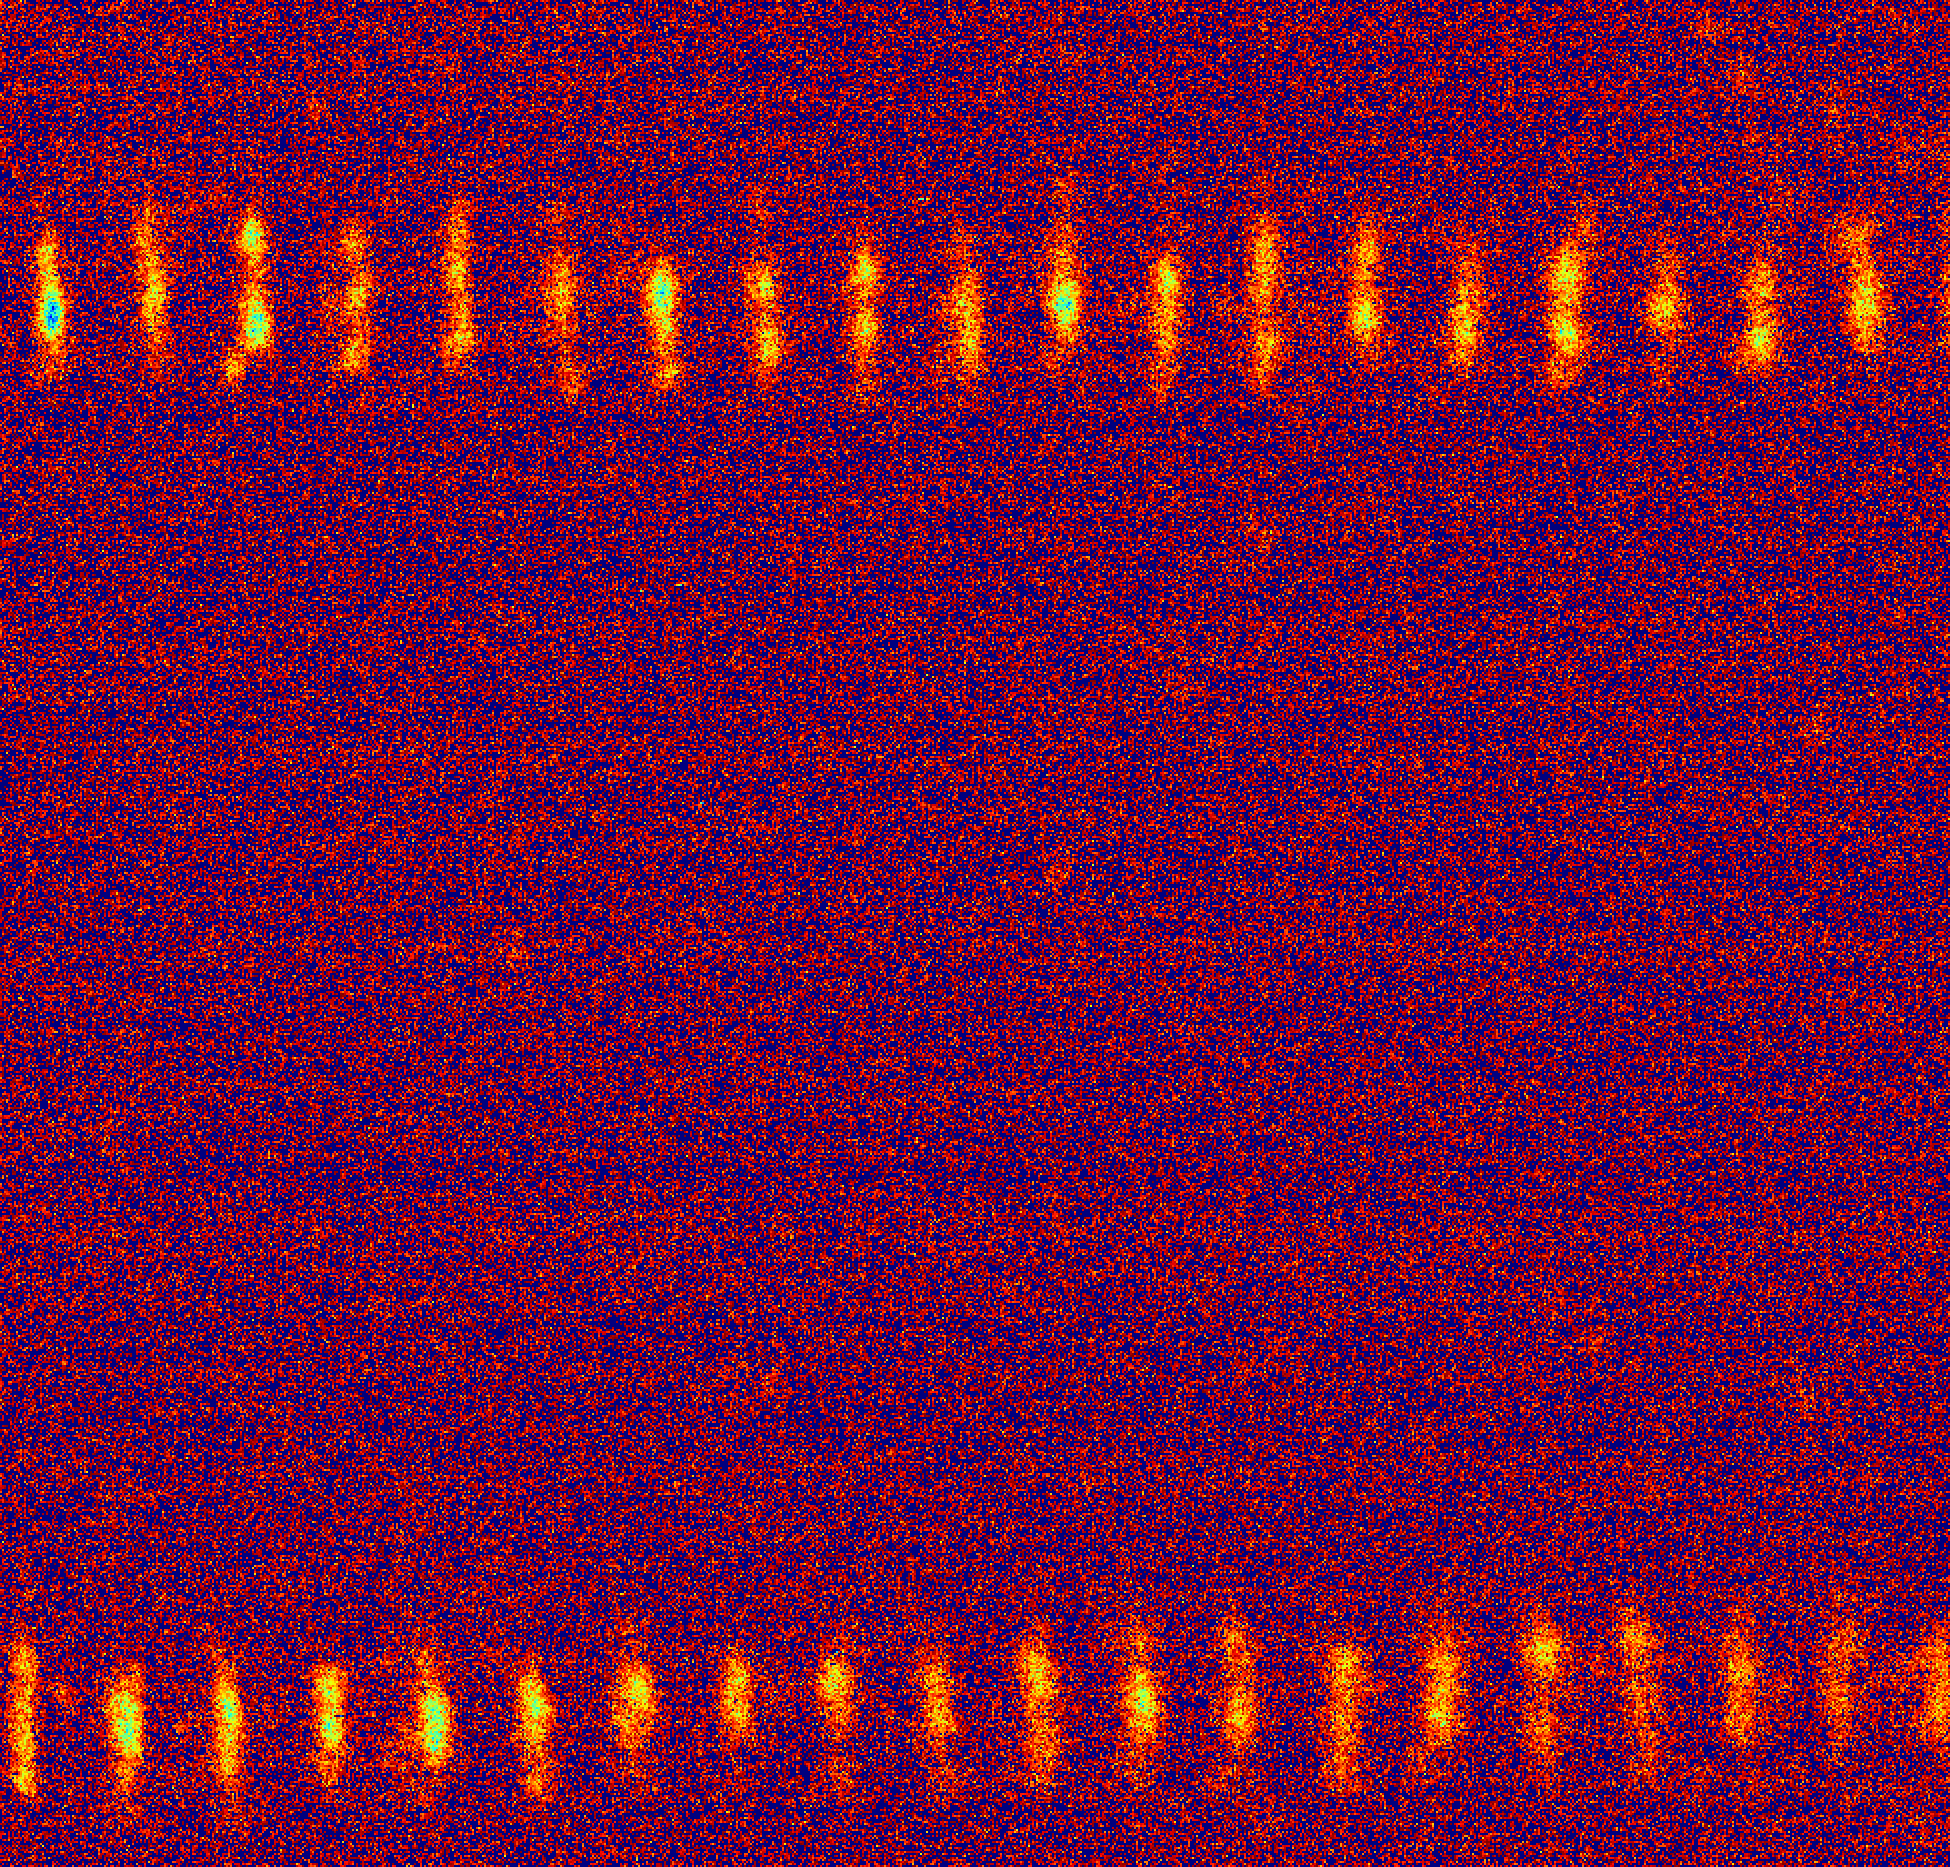
\includegraphics[height=100pt]{IP/analog10sx50_backgroundsubstractedcrop.pdf}}
};
\node at (5.5,2) {\fbox{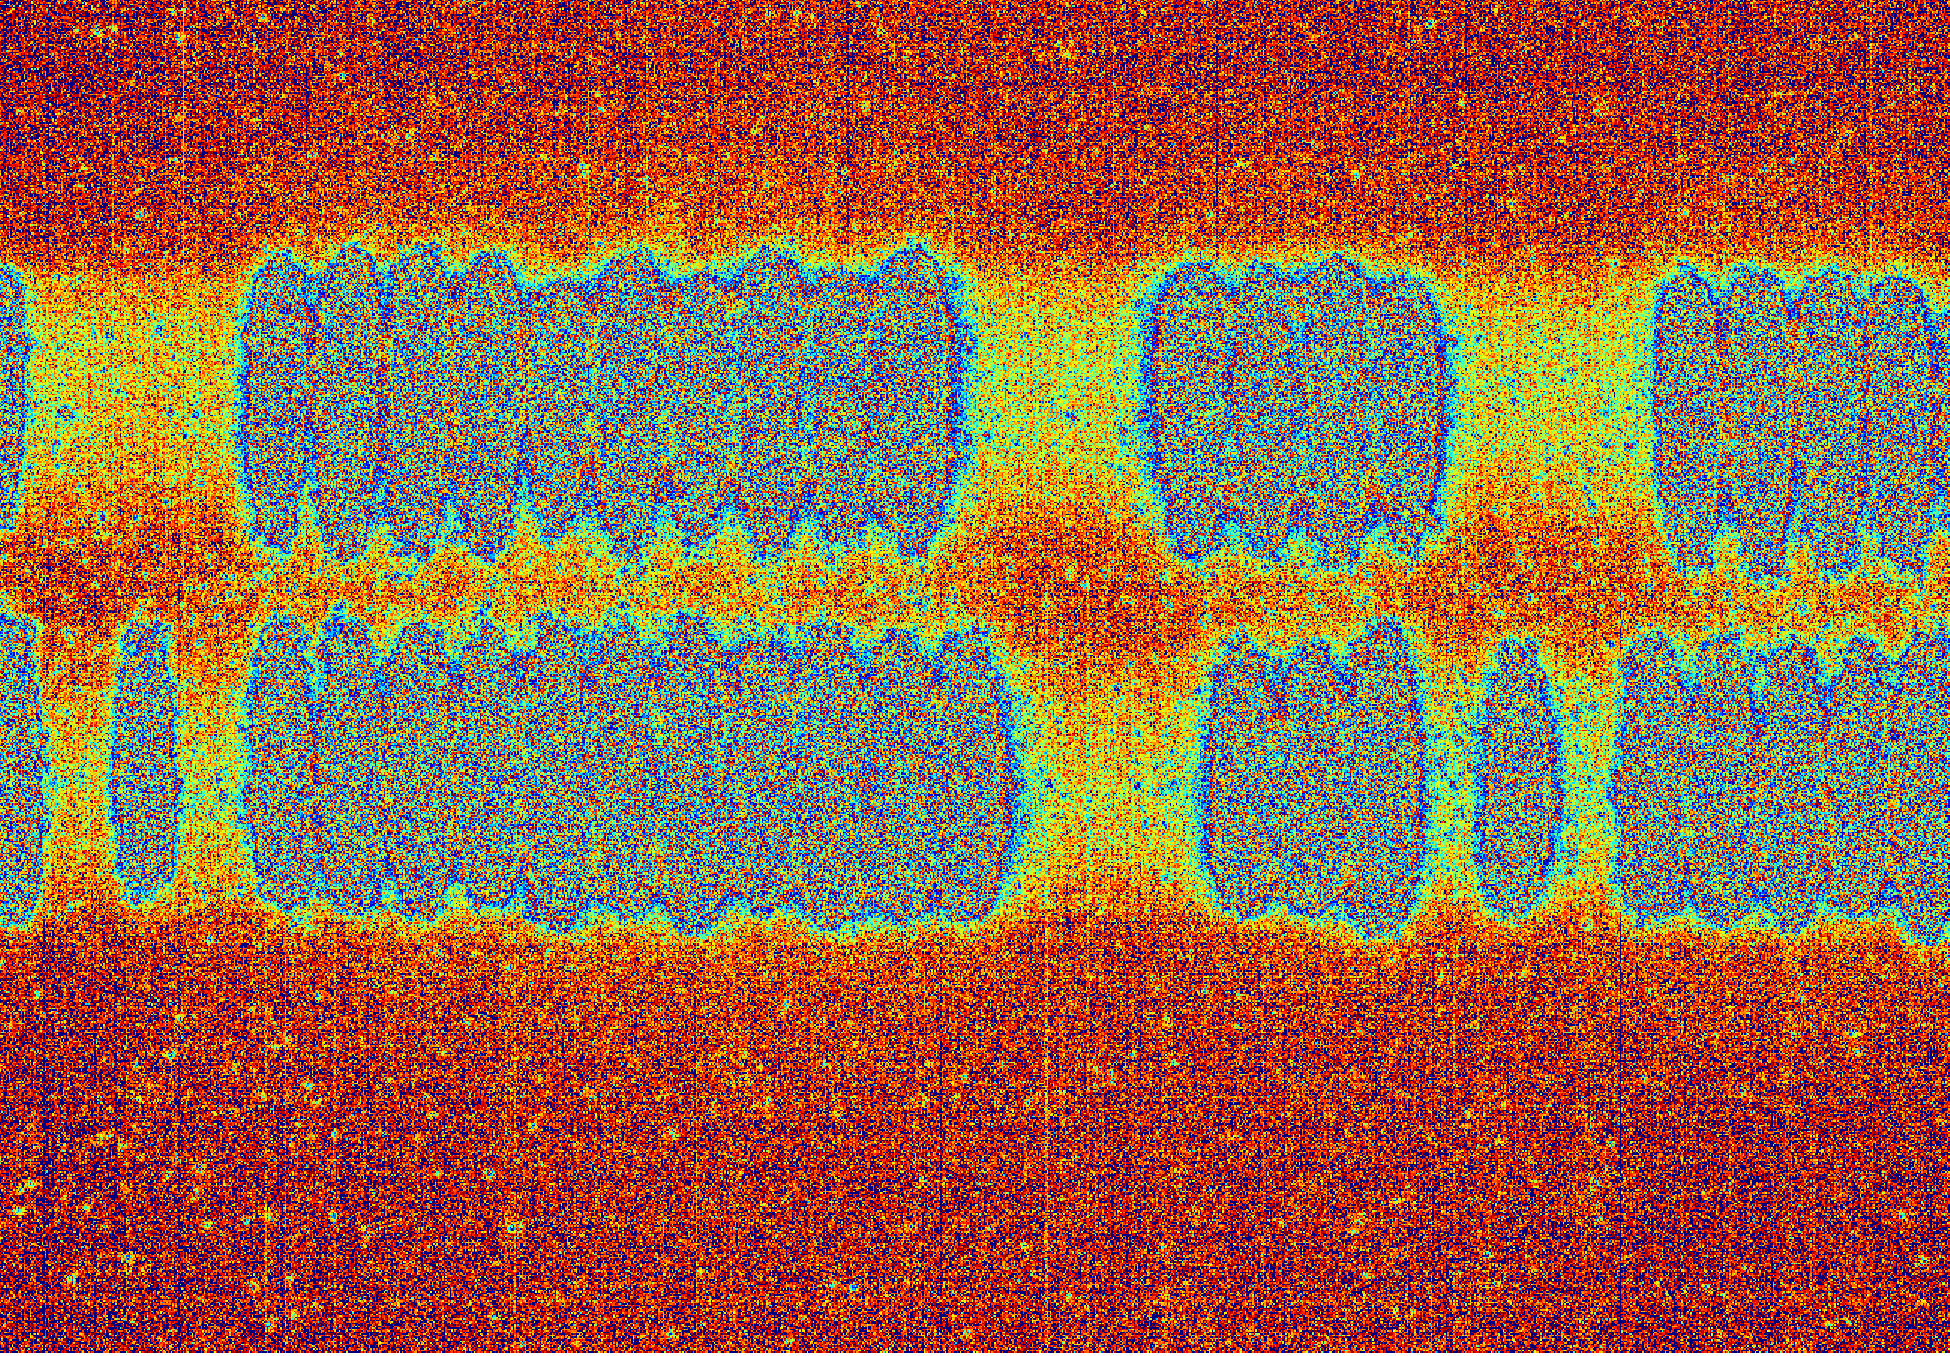
\includegraphics[height=100pt]{IP/lowalpha_100mA_zerisseneFuellungmitLueckecrop.pdf}}
};
\node at (11,3.3) {\fbox{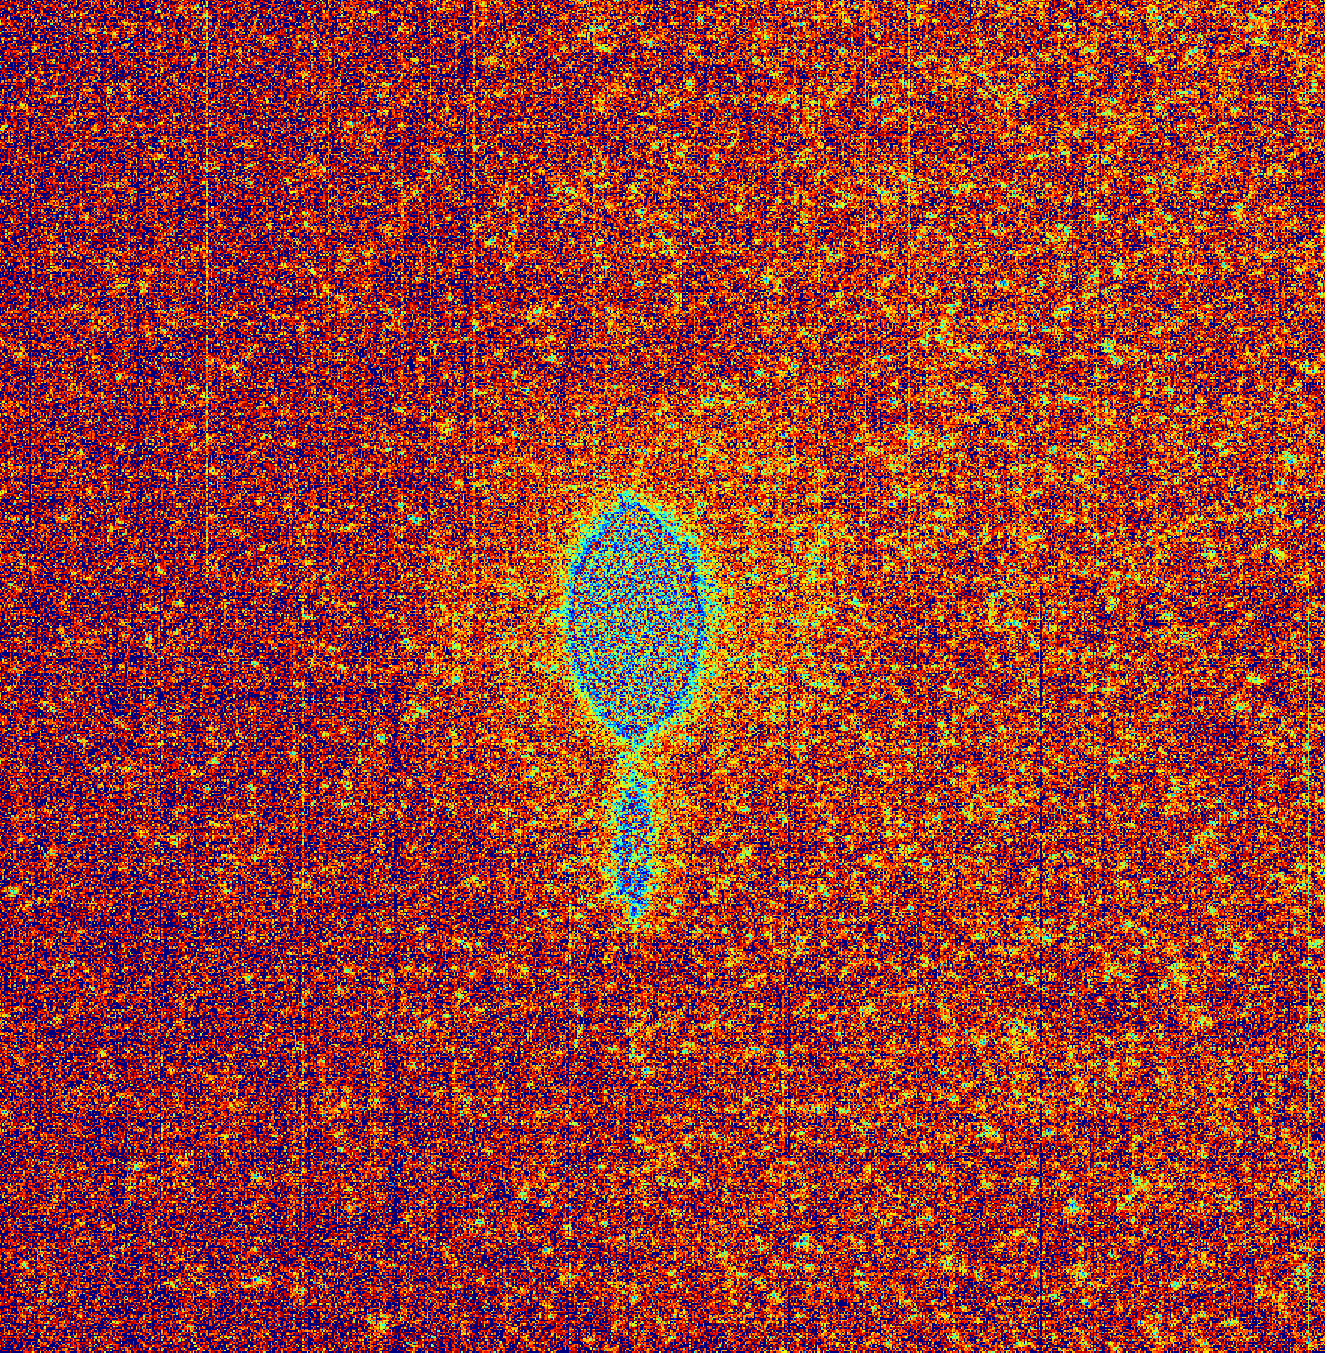
\includegraphics[height=100pt]{IP/lowalpha_1uAcrop.pdf}}
};
\node at (1,5.5) {
\large old camera, horizontal bunch length
};
\node at (5.5,4.2) {
\large new camera, horizontal bunch length
};
\node at (10.8,5.5) {
\large single bunch measurement
};
\draw[thick] (3,1.4) to [out=-90,in=180] (3.5,-0.3);
\draw[thick] (6.55,1.4) to [out=-90,in=0] (6.1,-0.3);
\node at (4.82,-0.3) { \large one revolution
};
\node at (11,-1.5) {
\includegraphics[width=2cm]{Pics/qrcode.pdf}};
\node at (11,-0.5) {
\begin{varwidth}{3cm}
tune resonance program source code
\end{varwidth}
};
\end{tikzpicture}
}

\headerbox{Tune Resonance Program}{name=tunediag,below=introbox,column=2,row=1,span=1,above=bottom}
{
{\color{hzbblue}\bf\large Details \& Features}
\begin{itemize}

\item[\color{hzbblue}\textbullet] developed in python
\item[\color{hzbblue}\textbullet] contains GUI built with wxpython
\item[\color{hzbblue}\textbullet] integrated with EPICS through the use of pyepics
\item[\color{hzbblue}\textbullet] live mode that displays current non-integer working point
\item[\color{hzbblue}\textbullet] given integer part, can display phase advance resonance lines and unit working point
\item[\color{hzbblue}\textbullet] various customizability options available

\end{itemize}
{\color{hzbblue}\bf\large Pictures \& Examples}
\begin{center}
\large Third order structural and phase advance resonance lines for the MLS
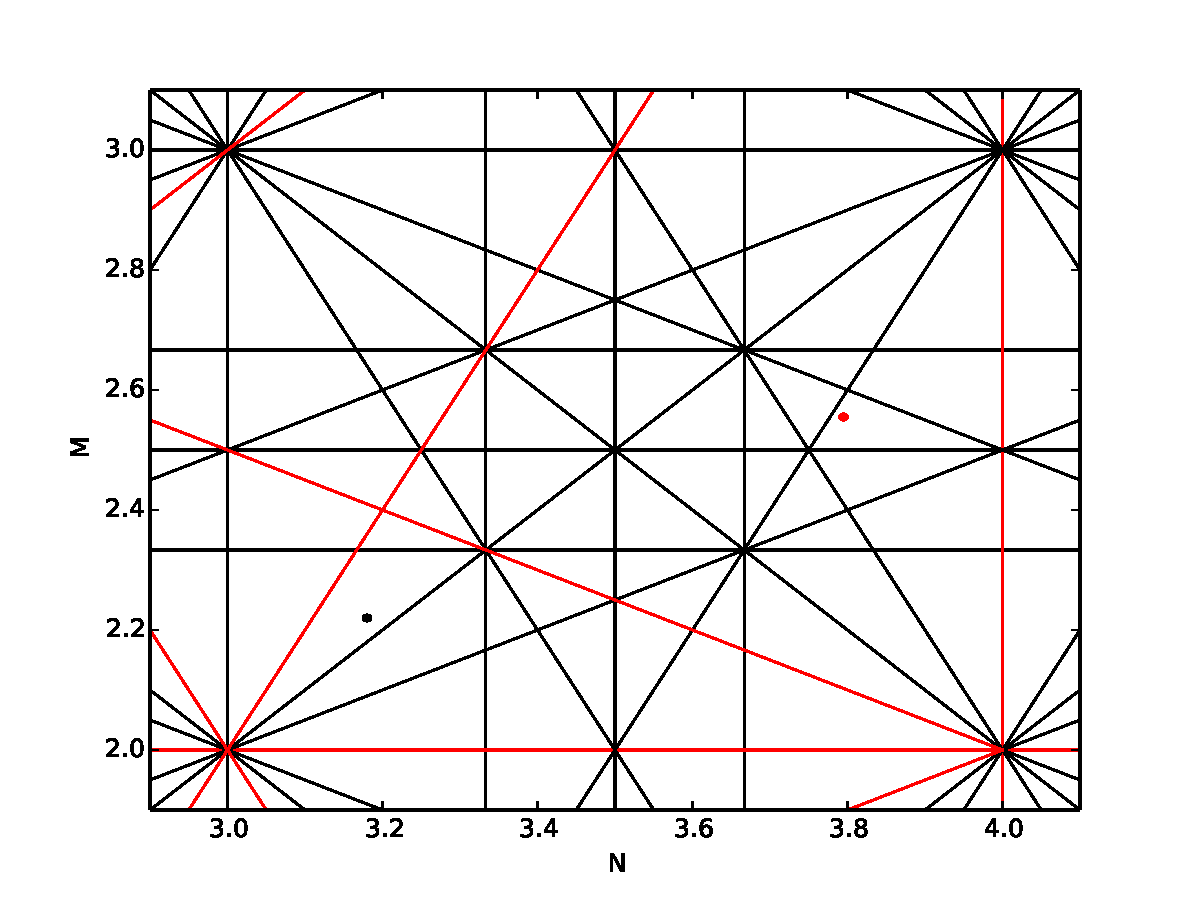
\includegraphics[width=200pt]{Pics/image.pdf}
\large Fifth order difference resonance lines ordered by color
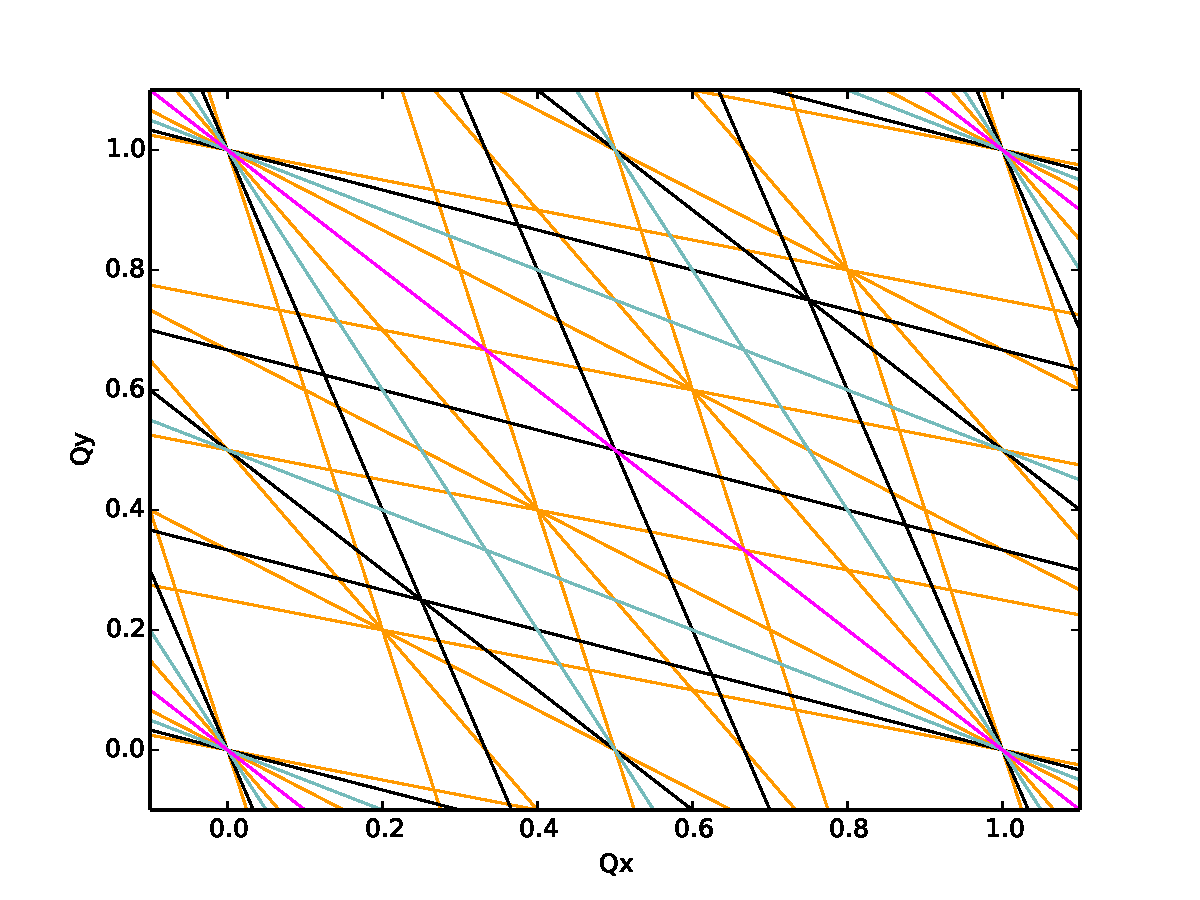
\includegraphics[width=200pt]{Pics/image2.pdf}
\end{center}

}
\end{poster}
\end{document}
